\documentclass[margin=5mm]{standalone}
\usepackage{pgfplots}
\usepgfplotslibrary{fillbetween} 
\usepackage{amsmath}
\begin{document}
	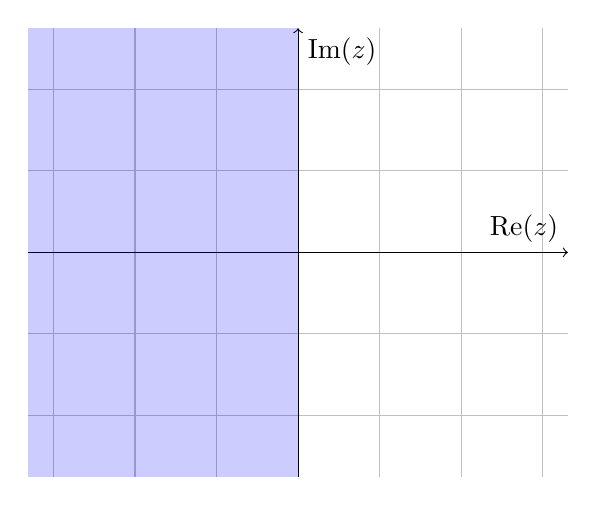
\begin{tikzpicture} 
		\begin{axis}[%
				axis x line=middle,    % put the x axis in the middle
				axis y line=middle,    % put the y axis in the middle
				axis line style={->},  % arrows on the axis
				xlabel={$\operatorname{Re}(z)$}, 			ylabel={$\operatorname{Im}(z)$},
				enlargelimits=0.05,
				grid,
				domain=-6:5.5,
				ymin = -5,
				ymax = 5,
				xmin = -5,
				xmax = 5,
				axis equal,
				ticks=none
			]
			\addplot[domain=-7:0, draw=none, fill=blue, fill opacity=0.2]{6} \closedcycle;
			\addplot[domain=-7:0, draw=none, fill=blue, fill opacity=0.2]{-6} \closedcycle;
		\end{axis} 
%		\node[above] at (current bounding box.north) {$|R(z)| = \left|\frac{1 + \frac{z}{2}}{1 - \frac{z}{2}} \right| \le 1$};
	\end{tikzpicture}
\end{document} 